\documentclass[11pt]{article}
\usepackage[a4paper,margin=1in]{geometry}
\usepackage[T1]{fontenc}
\usepackage[utf8]{inputenc}
\usepackage{lmodern}
\usepackage{hyperref}
\usepackage{enumitem}
\usepackage{booktabs}
\usepackage{pgfplots}
\pgfplotsset{compat=1.18}

\title{Omura Whitepaper}
\author{Omura Protocal}
\date{\today}

\begin{document}
\maketitle

\begin{abstract}
Omura is a multimodal search and indexing backend for Walrus-protocol blobs.
It provides scalable discovery, embedding, indexing, and retrieval workflows
for text, image, and mixed-content search.
\end{abstract}

\section{Introduction}
Omura addresses a simple problem: large blob ecosystems need fast and reliable
search over heterogeneous content. The platform combines blockchain-driven blob
discovery with modern embedding-based retrieval to support practical search APIs.

\section{Problem Statement}
\begin{itemize}[leftmargin=1.2em]
  \item Blob content is large, diverse, and continuously changing.
  \item Keyword-only search fails for multimodal and semantic use cases.
  \item Operators need production APIs and reproducible benchmarking.
\end{itemize}

\section{System Overview}
The Omura stack includes:
\begin{itemize}[leftmargin=1.2em]
  \item \textbf{Discovery Layer}: finds and tracks Walrus blobs over time.
  \item \textbf{Embedding Layer}: generates vector representations with the Omura Emmbed model.
  \item \textbf{Index Layer}: stores vectors and metadata for low-latency retrieval.
  \item \textbf{API Layer}: exposes search, blob, and stats endpoints.
\end{itemize}

\section{Omura\_emebd Model Design}
\subsection{Lineage and Fork Strategy}
The \texttt{omura\_emebd} embedding model is a forked deployment line built from
the SigLIP2 family, adapted for Omura retrieval workflows. In practice:
\begin{itemize}[leftmargin=1.2em]
  \item Base architecture and multimodal embedding behavior originate from SigLIP2.
  \item Omura-specific model packaging, naming, and deployment are versioned under
  \texttt{immortaltatsu/omura\_emebd}.
  \item Runtime integration is tuned for production search endpoints and benchmark reproducibility.
\end{itemize}

\subsection{How Embeddings Are Computed}
For both text and image inputs, the inference pipeline follows:
\begin{enumerate}[leftmargin=1.2em]
  \item Input normalization (text cleanup, image decoding/resize policy).
  \item Tokenization / processor encoding.
  \item Transformer forward pass on GPU (or CPU fallback).
  \item Feature extraction from model output.
  \item L2 normalization to produce unit-length vectors for cosine similarity.
\end{enumerate}

Given vector output \(v \in \mathbb{R}^{d}\), Omura uses:
\[
\hat{v} = \frac{v}{\|v\|_2}
\]
and similarity between query \(q\) and candidate \(x\):
\[
\mathrm{sim}(q, x) = \hat{q}^{\top}\hat{x}
\]
This keeps scoring stable across modalities and enables efficient nearest-neighbor retrieval.

\subsection{Document and Query Behavior}
\begin{itemize}[leftmargin=1.2em]
  \item \textbf{Short query mode}: a single vector is produced for low-latency search.
  \item \textbf{Document mode}: long text can be chunked, embedded per chunk, then averaged and renormalized.
  \item \textbf{Image mode}: image features are extracted with the same embedding backbone for cross-modal retrieval.
\end{itemize}

\subsection{Operational Advantages of the Fork}
The forked \texttt{omura\_emebd} line gives Omura:
\begin{itemize}[leftmargin=1.2em]
  \item Controlled model identity and release lifecycle.
  \item Consistent benchmark target across environments.
  \item A direct path to tune prompts, preprocessing, and retrieval behavior without changing the external API.
\end{itemize}

\section{Benchmarking Methodology}
Omura benchmark scripts are isolated in a standalone benchmark repository.
Key benchmark dimensions:
\begin{itemize}[leftmargin=1.2em]
  \item Initialization latency
  \item Throughput (items/second)
  \item Latency (ms/item)
  \item Retrieval quality (Recall@K, including Recall@10)
\end{itemize}

\section{Benchmark Results}
This section summarizes recent benchmark outputs from:
\begin{itemize}[leftmargin=1.2em]
  \item \texttt{benchmarks/results/repro\_run1.json}
  \item \texttt{benchmarks/results/repro\_run2.json}
  \item \texttt{benchmarks/results/repro\_recall10.json}
  \item \texttt{benchmarks/results/coco\_retrieval\_1k.json}
  \item \texttt{benchmarks/results/coco\_activation\_atlas\_1k\_stats.json}
\end{itemize}

\subsection{Reproducibility Snapshot}
\begin{table}[h]
\centering
\begin{tabular}{lrr}
\toprule
Metric & Run 1 & Run 2 \\
\midrule
Init seconds & 15.189 & 10.191 \\
Throughput (items/s) & 81.442 & 78.573 \\
Latency (ms/item) & 12.279 & 12.727 \\
Recall@1 & 1.000 & 1.000 \\
\bottomrule
\end{tabular}
\caption{Two identical benchmark runs show stable retrieval quality and expected runtime variance.}
\end{table}

\begin{center}
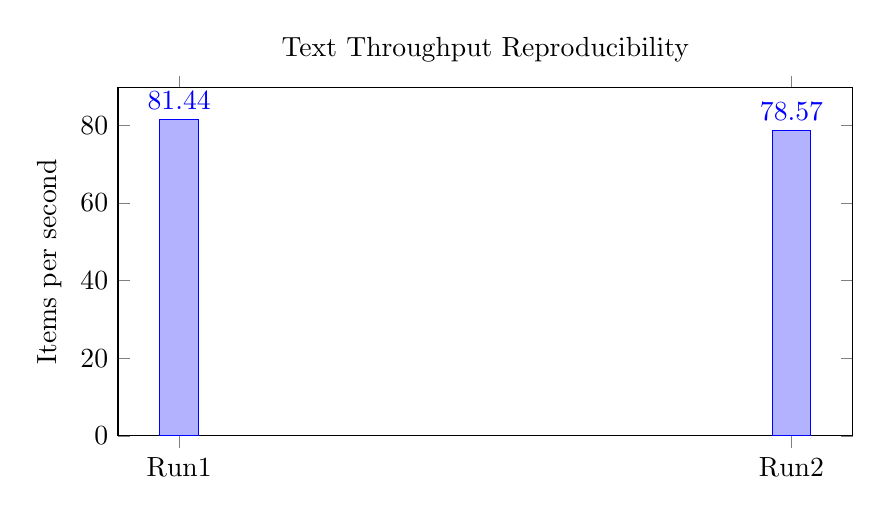
\begin{tikzpicture}
\begin{axis}[
    ybar,
    width=0.9\textwidth,
    height=6cm,
    bar width=14pt,
    ymin=0,
    ylabel={Items per second},
    symbolic x coords={Run1,Run2},
    xtick=data,
    nodes near coords,
    title={Text Throughput Reproducibility}
]
\addplot coordinates {(Run1,81.442) (Run2,78.573)};
\end{axis}
\end{tikzpicture}
\end{center}

\subsection{Retrieval Quality (Recall@K)}
On the fresh COCO 1k run (\(1000\) images, \(5000\) captions), measured text-to-image recall is:
\begin{itemize}[leftmargin=1.2em]
  \item \(R@1 = 0.0036\)
  \item \(R@5 = 0.0212\)
  \item \(R@10 = 0.0368\)
\end{itemize}

\begin{center}
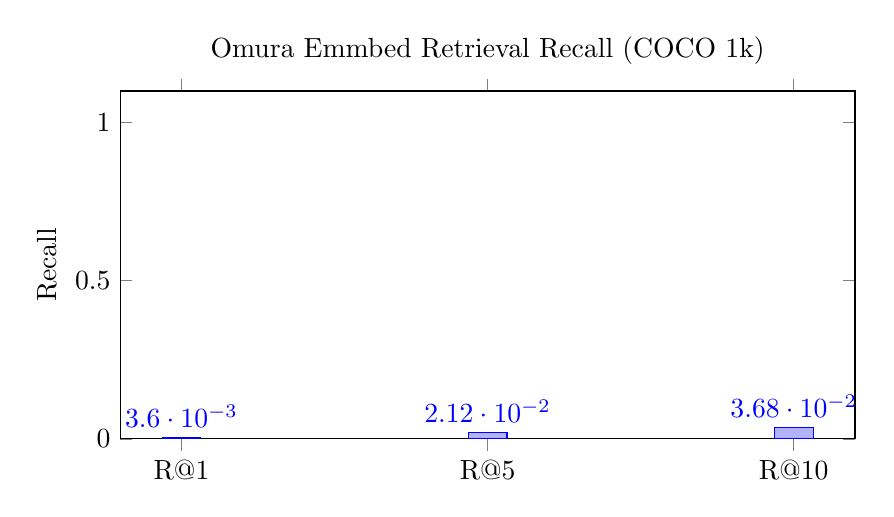
\begin{tikzpicture}
\begin{axis}[
    ybar,
    width=0.9\textwidth,
    height=6cm,
    bar width=14pt,
    ymin=0,
    ymax=1.1,
    ylabel={Recall},
    symbolic x coords={R@1,R@5,R@10},
    xtick=data,
    nodes near coords,
    title={Omura Emmbed Retrieval Recall (COCO 1k)}
]
\addplot coordinates {(R@1,0.0036) (R@5,0.0212) (R@10,0.0368)};
\end{axis}
\end{tikzpicture}
\end{center}

\section{COCO Activation Atlas Analysis}
This atlas section refers to benchmark-time analysis on COCO-style image/caption data,
not Walrus production traffic. We generated a PCA-based activation atlas from \(1000\)
image embeddings and saved it as:
\begin{itemize}[leftmargin=1.2em]
  \item \texttt{benchmarks/results/coco\_activation\_atlas\_1k.png}
\end{itemize}

The corresponding real run statistics are:
\begin{itemize}[leftmargin=1.2em]
  \item Num points: \(1000\)
  \item Embedding dim: \(768\)
  \item PC1 std: \(0.1591\)
  \item PC2 std: \(0.1405\)
\end{itemize}

\begin{center}
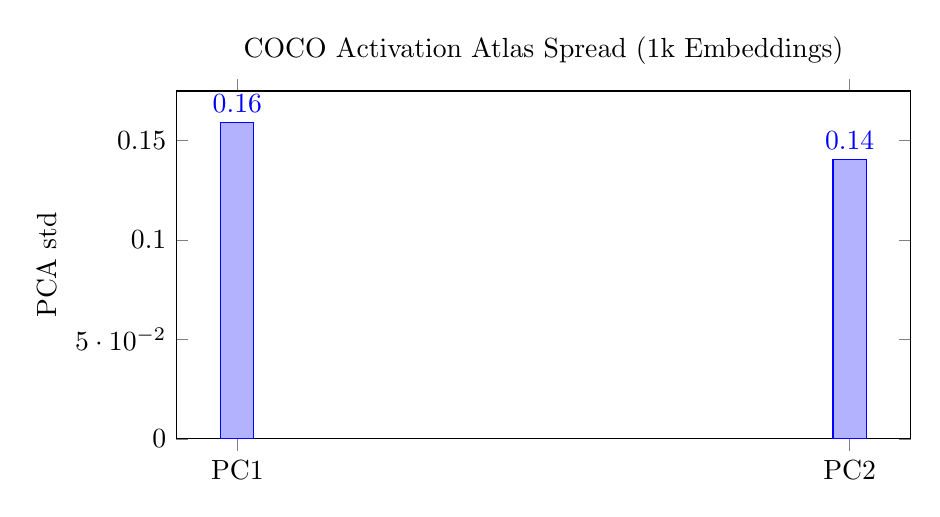
\begin{tikzpicture}
\begin{axis}[
    ybar,
    width=0.9\textwidth,
    height=6cm,
    bar width=12pt,
    ymin=0,
    ylabel={PCA std},
    symbolic x coords={PC1,PC2},
    xtick=data,
    nodes near coords,
    title={COCO Activation Atlas Spread (1k Embeddings)}
]
\addplot coordinates {
    (PC1,0.1591)
    (PC2,0.1405)
};
\end{axis}
\end{tikzpicture}
\end{center}

These atlas charts are used to interpret benchmark behavior (coverage, class skew,
and retrieval balance). They should not be read as live Walrus-network distribution.

\subsection{Zero-Shot Classification and Flagging}
Omura uses a zero-shot semantic approach for lightweight classification and safety
flagging without task-specific supervised retraining:
\begin{itemize}[leftmargin=1.2em]
  \item \textbf{Category Anchors}: textual prompts (e.g., \texttt{cat}, \texttt{dog},
  \texttt{human}, \texttt{scenery\_landscape}) are embedded into the same vector
  space as image embeddings.
  \item \textbf{Nearest-Anchor Assignment}: each image vector is compared via cosine
  similarity to anchor vectors and assigned to the closest category.
  \item \textbf{NSFW Prototypes}: dedicated safety prompts are embedded as NSFW
  prototypes; image-to-prototype similarity is converted into a safety score.
  \item \textbf{Flagging Rule}: content is flagged when the safety score exceeds a
  configurable threshold (default operational threshold: \(>85\) on a 0--100 scale).
\end{itemize}

This approach keeps the classifier interpretable, low-overhead, and easy to retune
by editing prompts and thresholds rather than retraining model weights.

\section{Impact on Private Search Engines}
The same retrieval design materially changes how private search engines can be built
and operated:
\begin{itemize}[leftmargin=1.2em]
  \item \textbf{Privacy-Preserving by Deployment Choice}: embeddings and nearest-neighbor
  retrieval can run inside private infrastructure, reducing dependence on external
  query-time APIs.
  \item \textbf{Semantic Search Without Labeling Programs}: zero-shot category anchors
  allow operators to ship useful semantic filtering and routing without collecting
  large labeled datasets.
  \item \textbf{Fast Policy Iteration}: safety and relevance behavior can be tuned by
  adjusting prompts and thresholds, avoiding expensive full-model retraining cycles.
  \item \textbf{Unified Multimodal Index}: text and image search share one similarity
  space, simplifying infrastructure for mixed-content archives.
  \item \textbf{Auditable Decisions}: cosine-similarity scoring and explicit anchors make
  ranking and flagging easier to inspect than opaque end-to-end classifiers.
\end{itemize}

In practical terms, this enables private search products to move from
``keyword + manual rules'' toward controllable semantic retrieval while maintaining
data residency, predictable costs, and operational transparency.

\section{End-to-End Technical Pipeline}
\subsection{Ingestion and Discovery}
Omura continuously discovers blobs, tracks lifecycle state (active/expired), and
stores canonical metadata required for retrieval and governance. The ingestion path
is designed for eventual consistency: ingestion can proceed while indexing catches up,
and search can continue with the latest committed vector state.

\subsection{Parsing and Modality Detection}
Incoming payloads are routed through lightweight modality detection and parsers:
\begin{itemize}[leftmargin=1.2em]
  \item Binary/image payloads are normalized into visual tensors.
  \item Text payloads are cleaned, chunked, and prepared for document embedding.
  \item Unsupported or ambiguous payloads are retained in metadata and can be
  reprocessed later as parsers improve.
\end{itemize}

\subsection{Embedding and Feature Standardization}
All vectors are normalized and persisted with metadata pointers. Standardization rules:
\begin{itemize}[leftmargin=1.2em]
  \item Unit-norm vectors for cosine-compatible scoring.
  \item Stable embedding dimensions at write-time.
  \item Deterministic preprocessing for benchmark reproducibility.
\end{itemize}

\subsection{Index Construction}
Indexing is performed over the active embedding set. Omura maintains:
\begin{itemize}[leftmargin=1.2em]
  \item Metadata store for blob attributes, safety status, and routing context.
  \item Vector index for approximate or exact nearest-neighbor retrieval.
  \item Rebuild hooks to refresh safety flags and semantic labels as policies evolve.
\end{itemize}

\subsection{Query Execution}
At query time:
\begin{enumerate}[leftmargin=1.2em]
  \item Query text (or image) is embedded in the same vector space.
  \item Similarity search retrieves top candidates.
  \item Policy filters are applied (safety flags, modality, active-state constraints).
  \item Results are scored, ranked, and returned with metadata for downstream UX.
\end{enumerate}

\section{Retrieval and Ranking Mechanics}
\subsection{Similarity Core}
Omura uses normalized dot product (cosine) as the canonical similarity operator.
For candidate set \(\mathcal{D}\), ranking is:
\[
\operatorname*{arg\,topK}_{x \in \mathcal{D}} \hat{q}^{\top}\hat{x}
\]
where \(\hat{q}\) and \(\hat{x}\) are L2-normalized vectors.

\subsection{Document Chunk Aggregation}
Long documents are embedded as chunk vectors \(\{d_i\}_{i=1}^{n}\). A document
representation is computed as:
\[
\bar{d} = \frac{1}{n}\sum_{i=1}^{n} d_i,\qquad \hat{d}=\frac{\bar{d}}{\|\bar{d}\|_2}
\]
This improves retrieval stability for long-form content while keeping query-time
latency bounded.

\subsection{Safety-Aware Ranking}
Safety scoring and semantic filtering are integrated as first-class constraints:
\begin{itemize}[leftmargin=1.2em]
  \item Hard filter mode excludes flagged content.
  \item Soft filter mode down-ranks flagged content while preserving recall for audit tools.
  \item Thresholds are policy-controlled and environment-specific.
\end{itemize}

\section{Benchmark Framework and Reproducibility}
\subsection{Repository Separation}
Omura isolates benchmark code from backend runtime code. This provides:
\begin{itemize}[leftmargin=1.2em]
  \item Cleaner dependency boundaries.
  \item Reproducible benchmark environments.
  \item Independent release cadence for evaluation tooling.
\end{itemize}

\subsection{Measured Dimensions}
The benchmark framework reports:
\begin{itemize}[leftmargin=1.2em]
  \item cold-start initialization time,
  \item per-item latency and throughput,
  \item retrieval metrics \(R@1, R@5, R@10\),
  \item reproducibility deltas across repeated runs.
\end{itemize}

\subsection{Interpretation Guidance}
When comparing runs:
\begin{itemize}[leftmargin=1.2em]
  \item Prioritize recall stability first.
  \item Treat throughput variance as expected under shared GPU workloads.
  \item Track trends over multiple runs rather than single-run outliers.
\end{itemize}

\section{Production Deployment Model}
\subsection{Service Topology}
A typical production topology includes:
\begin{itemize}[leftmargin=1.2em]
  \item API service (request handling, auth, policy),
  \item indexer worker (embedding and indexing),
  \item metadata database,
  \item vector index storage.
\end{itemize}

\subsection{Operational Controls}
Recommended controls:
\begin{itemize}[leftmargin=1.2em]
  \item Request budget limits (payload size, timeout, concurrency).
  \item Backpressure and queueing for indexing workloads.
  \item Periodic index integrity checks and recovery playbooks.
  \item Version pinning for model, processor, and benchmark scripts.
\end{itemize}

\section{Limitations and Trade-offs}
\begin{itemize}[leftmargin=1.2em]
  \item Zero-shot anchors are prompt-sensitive and require periodic calibration.
  \item Small benchmark suites can overestimate generalization quality.
  \item Similarity-only retrieval can miss task-specific intent without reranking.
  \item Safety thresholds trade false positives against false negatives.
\end{itemize}

\section{Future Technical Work}
\begin{itemize}[leftmargin=1.2em]
  \item Add larger-scale benchmark corpora and multilingual suites.
  \item Introduce optional reranking layers for intent-sensitive use cases.
  \item Publish model-card style evaluation deltas per release.
  \item Expand policy tooling for enterprise private-search deployments.
\end{itemize}

\section{Security and Operational Notes}
\begin{itemize}[leftmargin=1.2em]
  \item Keep private keys and API credentials out of source control.
  \item Enforce rate limits and payload-size constraints on public APIs.
  \item Monitor embedding/index drift and benchmark reproducibility over releases.
\end{itemize}

\section{Roadmap}
\begin{itemize}[leftmargin=1.2em]
  \item Expand benchmark suites and public result dashboards.
  \item Improve retrieval relevance for multilingual and long-document workloads.
  \item Publish periodic model and system evaluation reports.
\end{itemize}

\section{Conclusion}
Omura provides a practical foundation for multimodal blob indexing and search.
Its separation of backend and benchmark repositories enables faster iteration
and clearer reproducibility for research and production teams.

\end{document}
